\documentclass[tikz, border=6pt]{standalone}
\usepackage[T1]{fontenc}
\usepackage{lmodern}
\usepackage{amsmath,amssymb,bm}
\usepackage[scaled=0.95]{helvet}
\usetikzlibrary{arrows.meta, calc}
\definecolor{Blue}{HTML}{3A76D8}
\definecolor{Green}{HTML}{3BA55C}
\definecolor{Orange}{HTML}{EE8133}
\definecolor{Red}{HTML}{DF4B4B}
\definecolor{Ink}{HTML}{1F2937}
\colorlet{input}{Green}
\colorlet{output}{Red}
\begin{document}
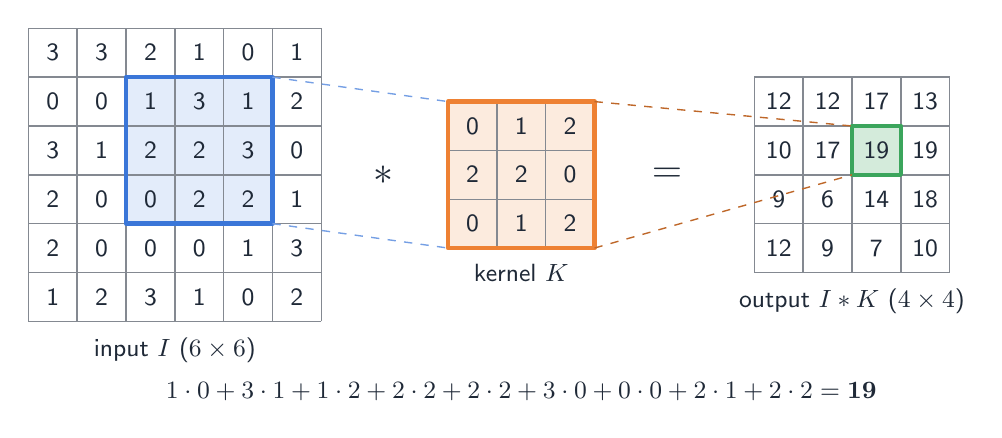
\begin{tikzpicture}[color=Ink, execute at begin picture={\sffamily}, line width=0.6pt, >={Stealth[length=5.5pt, width=4pt, inset=1.2pt]}, line join=round]
  % cell grid  6x6
  \fill[Blue!14] (-0.62,0.62) rectangle (0,1.24) (0,0.62) rectangle (0.62,1.24) (0.62,0.62) rectangle (1.24,1.24) (-0.62,0) rectangle (0,0.62) (0,0) rectangle (0.62,0.62) (0.62,0) rectangle (1.24,0.62) (-0.62,-0.62) rectangle (0,0) (0,-0.62) rectangle (0.62,0) (0.62,-0.62) rectangle (1.24,0);
  \draw[Ink!55, line width=0.5pt] (-1.86,-1.86) grid[step=0.62] (1.86,1.86);
  \node[font=\small, text=Ink, inner sep=0pt] at (-1.55,1.55) {3};
  \node[font=\small, text=Ink, inner sep=0pt] at (-0.93,1.55) {3};
  \node[font=\small, text=Ink, inner sep=0pt] at (-0.31,1.55) {2};
  \node[font=\small, text=Ink, inner sep=0pt] at (0.31,1.55) {1};
  \node[font=\small, text=Ink, inner sep=0pt] at (0.93,1.55) {0};
  \node[font=\small, text=Ink, inner sep=0pt] at (1.55,1.55) {1};
  \node[font=\small, text=Ink, inner sep=0pt] at (-1.55,0.93) {0};
  \node[font=\small, text=Ink, inner sep=0pt] at (-0.93,0.93) {0};
  \node[font=\small, text=Ink, inner sep=0pt] at (-0.31,0.93) {1};
  \node[font=\small, text=Ink, inner sep=0pt] at (0.31,0.93) {3};
  \node[font=\small, text=Ink, inner sep=0pt] at (0.93,0.93) {1};
  \node[font=\small, text=Ink, inner sep=0pt] at (1.55,0.93) {2};
  \node[font=\small, text=Ink, inner sep=0pt] at (-1.55,0.31) {3};
  \node[font=\small, text=Ink, inner sep=0pt] at (-0.93,0.31) {1};
  \node[font=\small, text=Ink, inner sep=0pt] at (-0.31,0.31) {2};
  \node[font=\small, text=Ink, inner sep=0pt] at (0.31,0.31) {2};
  \node[font=\small, text=Ink, inner sep=0pt] at (0.93,0.31) {3};
  \node[font=\small, text=Ink, inner sep=0pt] at (1.55,0.31) {0};
  \node[font=\small, text=Ink, inner sep=0pt] at (-1.55,-0.31) {2};
  \node[font=\small, text=Ink, inner sep=0pt] at (-0.93,-0.31) {0};
  \node[font=\small, text=Ink, inner sep=0pt] at (-0.31,-0.31) {0};
  \node[font=\small, text=Ink, inner sep=0pt] at (0.31,-0.31) {2};
  \node[font=\small, text=Ink, inner sep=0pt] at (0.93,-0.31) {2};
  \node[font=\small, text=Ink, inner sep=0pt] at (1.55,-0.31) {1};
  \node[font=\small, text=Ink, inner sep=0pt] at (-1.55,-0.93) {2};
  \node[font=\small, text=Ink, inner sep=0pt] at (-0.93,-0.93) {0};
  \node[font=\small, text=Ink, inner sep=0pt] at (-0.31,-0.93) {0};
  \node[font=\small, text=Ink, inner sep=0pt] at (0.31,-0.93) {0};
  \node[font=\small, text=Ink, inner sep=0pt] at (0.93,-0.93) {1};
  \node[font=\small, text=Ink, inner sep=0pt] at (1.55,-0.93) {3};
  \node[font=\small, text=Ink, inner sep=0pt] at (-1.55,-1.55) {1};
  \node[font=\small, text=Ink, inner sep=0pt] at (-0.93,-1.55) {2};
  \node[font=\small, text=Ink, inner sep=0pt] at (-0.31,-1.55) {3};
  \node[font=\small, text=Ink, inner sep=0pt] at (0.31,-1.55) {1};
  \node[font=\small, text=Ink, inner sep=0pt] at (0.93,-1.55) {0};
  \node[font=\small, text=Ink, inner sep=0pt] at (1.55,-1.55) {2};
  \draw[Blue, line width=1.6pt] (-0.62,-0.62) rectangle (1.24,1.24);
  \node[anchor=north, font=\small, align=center] at (0,-1.94) {input $I$ ($6\times 6$)};
  % cell grid  3x3
  \fill[Orange!16] (3.47,0.31) rectangle (4.09,0.93) (4.09,0.31) rectangle (4.71,0.93) (4.71,0.31) rectangle (5.33,0.93) (3.47,-0.31) rectangle (4.09,0.31) (4.09,-0.31) rectangle (4.71,0.31) (4.71,-0.31) rectangle (5.33,0.31) (3.47,-0.93) rectangle (4.09,-0.31) (4.09,-0.93) rectangle (4.71,-0.31) (4.71,-0.93) rectangle (5.33,-0.31);
  \draw[Ink!55, line width=0.5pt] (3.47,-0.93) -- (5.33,-0.93) (3.47,-0.31) -- (5.33,-0.31) (3.47,0.31) -- (5.33,0.31) (3.47,0.93) -- (5.33,0.93) (3.47,-0.93) -- (3.47,0.93) (4.09,-0.93) -- (4.09,0.93) (4.71,-0.93) -- (4.71,0.93) (5.33,-0.93) -- (5.33,0.93);
  \node[font=\small, text=Ink, inner sep=0pt] at (3.78,0.62) {0};
  \node[font=\small, text=Ink, inner sep=0pt] at (4.4,0.62) {1};
  \node[font=\small, text=Ink, inner sep=0pt] at (5.02,0.62) {2};
  \node[font=\small, text=Ink, inner sep=0pt] at (3.78,0) {2};
  \node[font=\small, text=Ink, inner sep=0pt] at (4.4,0) {2};
  \node[font=\small, text=Ink, inner sep=0pt] at (5.02,0) {0};
  \node[font=\small, text=Ink, inner sep=0pt] at (3.78,-0.62) {0};
  \node[font=\small, text=Ink, inner sep=0pt] at (4.4,-0.62) {1};
  \node[font=\small, text=Ink, inner sep=0pt] at (5.02,-0.62) {2};
  \draw[Orange, line width=1.6pt] (3.47,-0.93) rectangle (5.33,0.93);
  \node[anchor=north, font=\small, align=center] at (4.4,-1.01) {kernel $K$};
  % cell grid  4x4
  \fill[Green!22] (8.6,0) rectangle (9.22,0.62);
  \draw[Ink!55, line width=0.5pt] (7.36,-1.24) -- (9.84,-1.24) (7.36,-0.62) -- (9.84,-0.62) (7.36,0) -- (9.84,0) (7.36,0.62) -- (9.84,0.62) (7.36,1.24) -- (9.84,1.24) (7.36,-1.24) -- (7.36,1.24) (7.98,-1.24) -- (7.98,1.24) (8.6,-1.24) -- (8.6,1.24) (9.22,-1.24) -- (9.22,1.24) (9.84,-1.24) -- (9.84,1.24);
  \node[font=\small, text=Ink, inner sep=0pt] at (7.67,0.93) {12};
  \node[font=\small, text=Ink, inner sep=0pt] at (8.29,0.93) {12};
  \node[font=\small, text=Ink, inner sep=0pt] at (8.91,0.93) {17};
  \node[font=\small, text=Ink, inner sep=0pt] at (9.53,0.93) {13};
  \node[font=\small, text=Ink, inner sep=0pt] at (7.67,0.31) {10};
  \node[font=\small, text=Ink, inner sep=0pt] at (8.29,0.31) {17};
  \node[font=\small, text=Ink, inner sep=0pt] at (8.91,0.31) {19};
  \node[font=\small, text=Ink, inner sep=0pt] at (9.53,0.31) {19};
  \node[font=\small, text=Ink, inner sep=0pt] at (7.67,-0.31) {9};
  \node[font=\small, text=Ink, inner sep=0pt] at (8.29,-0.31) {6};
  \node[font=\small, text=Ink, inner sep=0pt] at (8.91,-0.31) {14};
  \node[font=\small, text=Ink, inner sep=0pt] at (9.53,-0.31) {18};
  \node[font=\small, text=Ink, inner sep=0pt] at (7.67,-0.93) {12};
  \node[font=\small, text=Ink, inner sep=0pt] at (8.29,-0.93) {9};
  \node[font=\small, text=Ink, inner sep=0pt] at (8.91,-0.93) {7};
  \node[font=\small, text=Ink, inner sep=0pt] at (9.53,-0.93) {10};
  \draw[Green, line width=1.6pt] (8.6,0) rectangle (9.22,0.62);
  \node[anchor=north, font=\small, align=center] at (8.6,-1.32) {output $I * K$ ($4\times 4$)};
  \draw[dashed, color=Blue!70, line width=0.5pt] (1.24,1.24) -- (3.47,0.93);
  \draw[dashed, color=Blue!70, line width=0.5pt] (1.24,-0.62) -- (3.47,-0.93);
  \draw[dashed, color=Orange!80!black, line width=0.5pt] (5.33,0.93) -- (8.6,0.62);
  \draw[dashed, color=Orange!80!black, line width=0.5pt] (5.33,-0.93) -- (8.6,0);
  \node[font=\Large] at (2.65,0) {$\ast$};
  \node[font=\Large] at (6.25,0) {$=$};
  \node[font=\small] at (4.4,-2.75) {$1\cdot0 + 3\cdot1 + 1\cdot2 + 2\cdot2 + 2\cdot2 + 3\cdot0 + 0\cdot0 + 2\cdot1 + 2\cdot2 = \mathbf{19}$};
\end{tikzpicture}
\end{document}
